\section{Interfaces in materials}

So far we have seen how much important the defects are to describe diffusion inside a solid state system, focussing on how defects allow it in the first place.  Still, we want now to look at a different type of defects that highly influences the diffusion and are \textbf{interfaces}. Basically, real materials are not a simple single block of atoms bonded together, but it's usually composed by chunks of the same material oriented in different directions, called \textbf{grains}, and the regions of space that separate them are the interfaces. We want to look into the description of such objects to see effectively their characteristic and how they influence the diffusion.

At first, we shall say that different types of interfaces exist depending on which type of material separates, like: crystal-vapor, crystal-liquid and crystal-crystal, that are possible to see in \figref{fig:Interfaces}. All of them are interesting and differ not only in the type of phase they connect. For example, it's possible to understand that the local degrees of freedom of such interfaces vary from one to another: in the first two types, in fact, having that liquid and vapor are isotropic then the interface is locally uniquely defined by the normal to the direction in which the interface point, which can be settled by two angles, so two degrees of freedom. On the other side, the crystal-crystal interface is more complex, since we need not only to describe the direction of the cut done by the interface, but also to describe the relative orientation of the two crystals in that position of space. A thing that can be done by imagining the two rotated respect one another, so that we can use the three Euler angle to define it, for a total of 5 degrees of freedom. In our study, we are going to account mainly for a specific type of interface that is defined as follows.
\dfn{Grain boundaries}
{
    A Homophasic interface between crystals with same structure and composition is called grain boundaries.
}
\noindent
Such a defect can be easily seen how describes a specific type of crystal-crystal interface, meaning that we will work in the most complex case with 5 macroscopic variable to work with.

\begin{figure}[b]
    \centering
    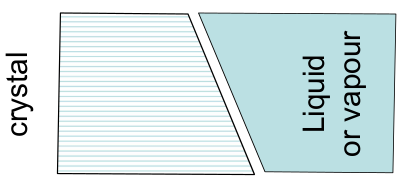
\includegraphics[width=0.4\textwidth]{Immagini/Crys-Liqu.png}
    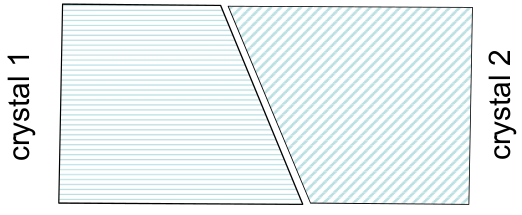
\includegraphics[width=0.4\textwidth]{Immagini/Crys-Crys.png}
    \caption
    {
        Simple image of crystal-liquid/vapor and crystal-crystal interface in order to graphically guide their description of the difference in the degrees of freedom.
    }
    \label{fig:Interfaces}
\end{figure}

Even after this simple description of what an interface is it's already possible to point out why they play a role in diffusive processes. In fact, interfaces can be seen as microscopically as regions of free space inside the material, where the atoms are able to jump from one position to another without the need of breaking bonds with all neighbors or moving all the atoms to pass through. Meaning that, the energy barrier that the processes posses is much lower near such defects, highly boosting the transition rate and, therefore, the diffusivity $D$. Experimental data, shown in \figref{fig:DiffusivityComp}, confirm these simple thoughts showing how the diffusivity of material has a great boost of also several order of magnitudes around interfaces. 
\begin{figure}[t]
    \centering
    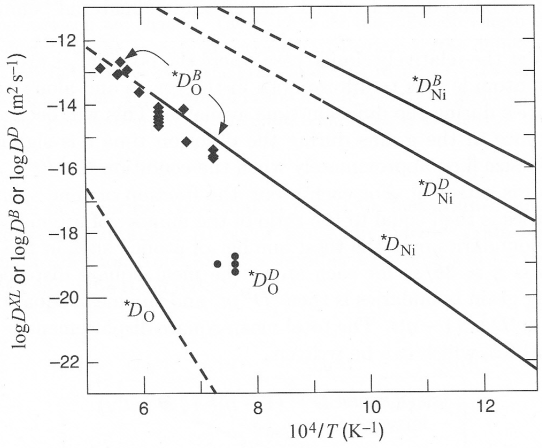
\includegraphics[width=0.4\textwidth]{Immagini/Dbound.png}
    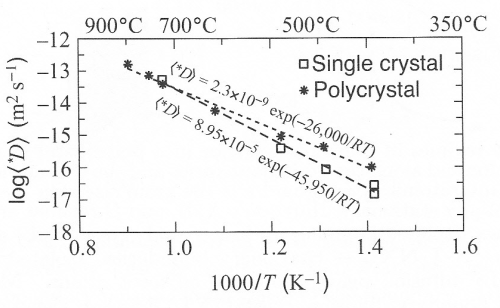
\includegraphics[width=0.55\textwidth]{Immagini/Dmean.png}
    \caption
    {
        Experimental data on the diffusivity value inside \ce{NiO}, with data for pure self-diffusion, $^*D$, diffusion near boundaries, $D^B$, and diffusion near dislocation, $D^D$, on the left. Then, on the right, data on the average value of the diffusivity in a pure single crystal vs a polycrystal which posses interface.
    }
    \label{fig:DiffusivityComp}
\end{figure}
Nevertheless, the average total value of the diffusivity, $D^{eff}$, does not change too much from a single crystal to one composed of grain boundaries and the reason is the following.
\thm{Effective diffusivity}
{
    Inside a polycrystal where the normal diffusivity is $D^{cry}$ and it's value on the boundaries is $D^B$ we will have that the total effective diffusivity is
    \begin{equation}
        D^{eff} = D + \frac{3\delta}{d_G}D^B,
    \end{equation}
    where $d_G$ is the grain size and $\delta$ the boundary thickness.
}
\pf{Proof}
{
    $D^{eff}$ is a weighted average between the pure $D^{cry}$ and $D^B$, where the weights are the relative extent of the volume where the two types of diffusion are active. Meaning that if we account that $V_B \ll V_{cry}$ we can write $V_T \approx V_{cry}$ and the weights are
    \begin{align}
        &w_{cry} = \frac{V_{cry}}{V_{cry}} = 1, &w_B = \frac{V_B}{V_{cry}},
    \end{align}
    where we can think at a grain as a sphere of diameter $d_G$ surrounded by an interface of thickness $\delta$. In this way we can write
    \begin{align}
        &V_B = \pi d_G^2 \delta, &V_{cry} = \frac{\pi}{6}d_G^3,
    \end{align}
    where we shall also take into account that the same interface is shared between two boundaries so that the total weight looks like the following
    \begin{equation}
        w_B = \frac{V_B}{2V_{cry}} = \frac{3\delta}{d_G}.
    \end{equation}
}
\noindent
Basically, due to the much smaller extensions of the interfaces inside the material the average diffusivity changes only partially respect to the incredible increase between $D$ and $D^B$. Still, the result is quite good, especially at lower temperatures since the exponent of $D^B$ is much smaller allowing for an enhancing of the total diffusion by also orders of magnitudes.

By such simple considerations we have already seen how interfaces can be a key point in the description of diffusion inside materials, giving a great boost to the performance overall. For this reason we aim into describing on a more precise level the main properties of such a defect, understanding how they are formed and modelling their evolution.

\nt
{
    Inside the description of surfaces during the course there was also another division between the category of crystal-crystal, defined by the way in which the interfaces are composed. In particular, they are divided between \textbf{sharp}, meaning that atoms form a precise line that divides the two boundaries creating a small interface tens of nanometers long, and \textbf{diffused}, where the interface is not really well-defined since the two phases that is connecting are kind of fused one into the other generating an interface that can be hundreds of nanometers in length.
}

\subsection{Surface free energy}